%!TEX program = xelatex
\documentclass[a4paper]{ctexart}

\usepackage{listings} 
\usepackage{geometry}
\usepackage{booktabs}
\usepackage{graphicx}
\usepackage{tabularx}
\usepackage{multirow}
\usepackage{enumitem}
\usepackage[bottom]{footmisc}

\renewcommand{\multirowsetup}{\centering}

\geometry{
    left=23mm,
    right=23mm,
    top=23mm,
    bottom=23mm,
}

\setlength{\parskip}{0.5em}

\title{\Huge PetLover 项目启动文档}

\author{
  项目成员:\\
  姬筠刚 191250055(PM)\\
  陈梓俊 191250016\\
  丁炳智 191250024\\
  刘庭烽 191250093\\
}
\date{\today}

\begin{document}

\maketitle

\centerline{
\includegraphics[]{logo.png}}

\newpage

\begin{abstract}
  本项目名为PetLover,是由本小组于2021年秋季学期《需求与商业模式创新》课程大作业中设计的软件产品项目。此文档为项目启动文档,主要内容包含项目简介、商业模式画布及其模块要点相关介绍。
\end{abstract}



\tableofcontents

\newpage

\setlength{\parskip}{1em}


\section{项目简介}
宠物,是当代社会人群必不可少的陪伴,无论是在外打拼的年轻人群体,还是安度晚年的老年人群体,抑或是中年人群体,都对宠物饲养有着或多或少的要求。由此,一些宠物交易市场和宠物日常交流平台应运而生。

经过一段时间的市场调研,我们发现:虽然目前市场上已存在宠物交易平台和宠物成长分享平台,但是能够提供一站式宠物服务(包括从宠物买卖、宠物饲养交流、宠物用品到宠物日常分享等的一系列相关服务)的软件平台少之又少。用户往往需要在平台A进行宠物交易,在平台B进行宠物用品购买,在平台C进行宠物疾病咨询,在平台D分享宠物日常……

为了避免宠物主人在各个平台之间“反复横跳”,我们计划打造一款集宠物(及相关用品)交易、宠物疾病咨询、宠物饲养教程、宠物日常分享四大功能于一身的宠物交流平台——PetLover平台(以下简称“PetLover”或“平台”),希望通过一站式服务真正地为宠物爱好者们提供便利;同时通过与各地线下实体宠物店、宠物医院等进行合作,建立全国各地的宠物交易/问诊线下网络,推进线上、线下双线模式的宠物交易和宠物疾病诊疗服务。

PetLover,帮助宠物爱好者们从头见证宠物宝贝的成长!


\section{度量数值}

本文档共包含了38个要点与18条关联关系。平均要点数量约为4个。要点的联系详见第三部分,每个联系之前有要点位置的标注,例如1a表示关键业务的第a条要点。

\section{商业模式画布}

\subsection{要点概述}

商业模式画布如下图

\begin{center}
  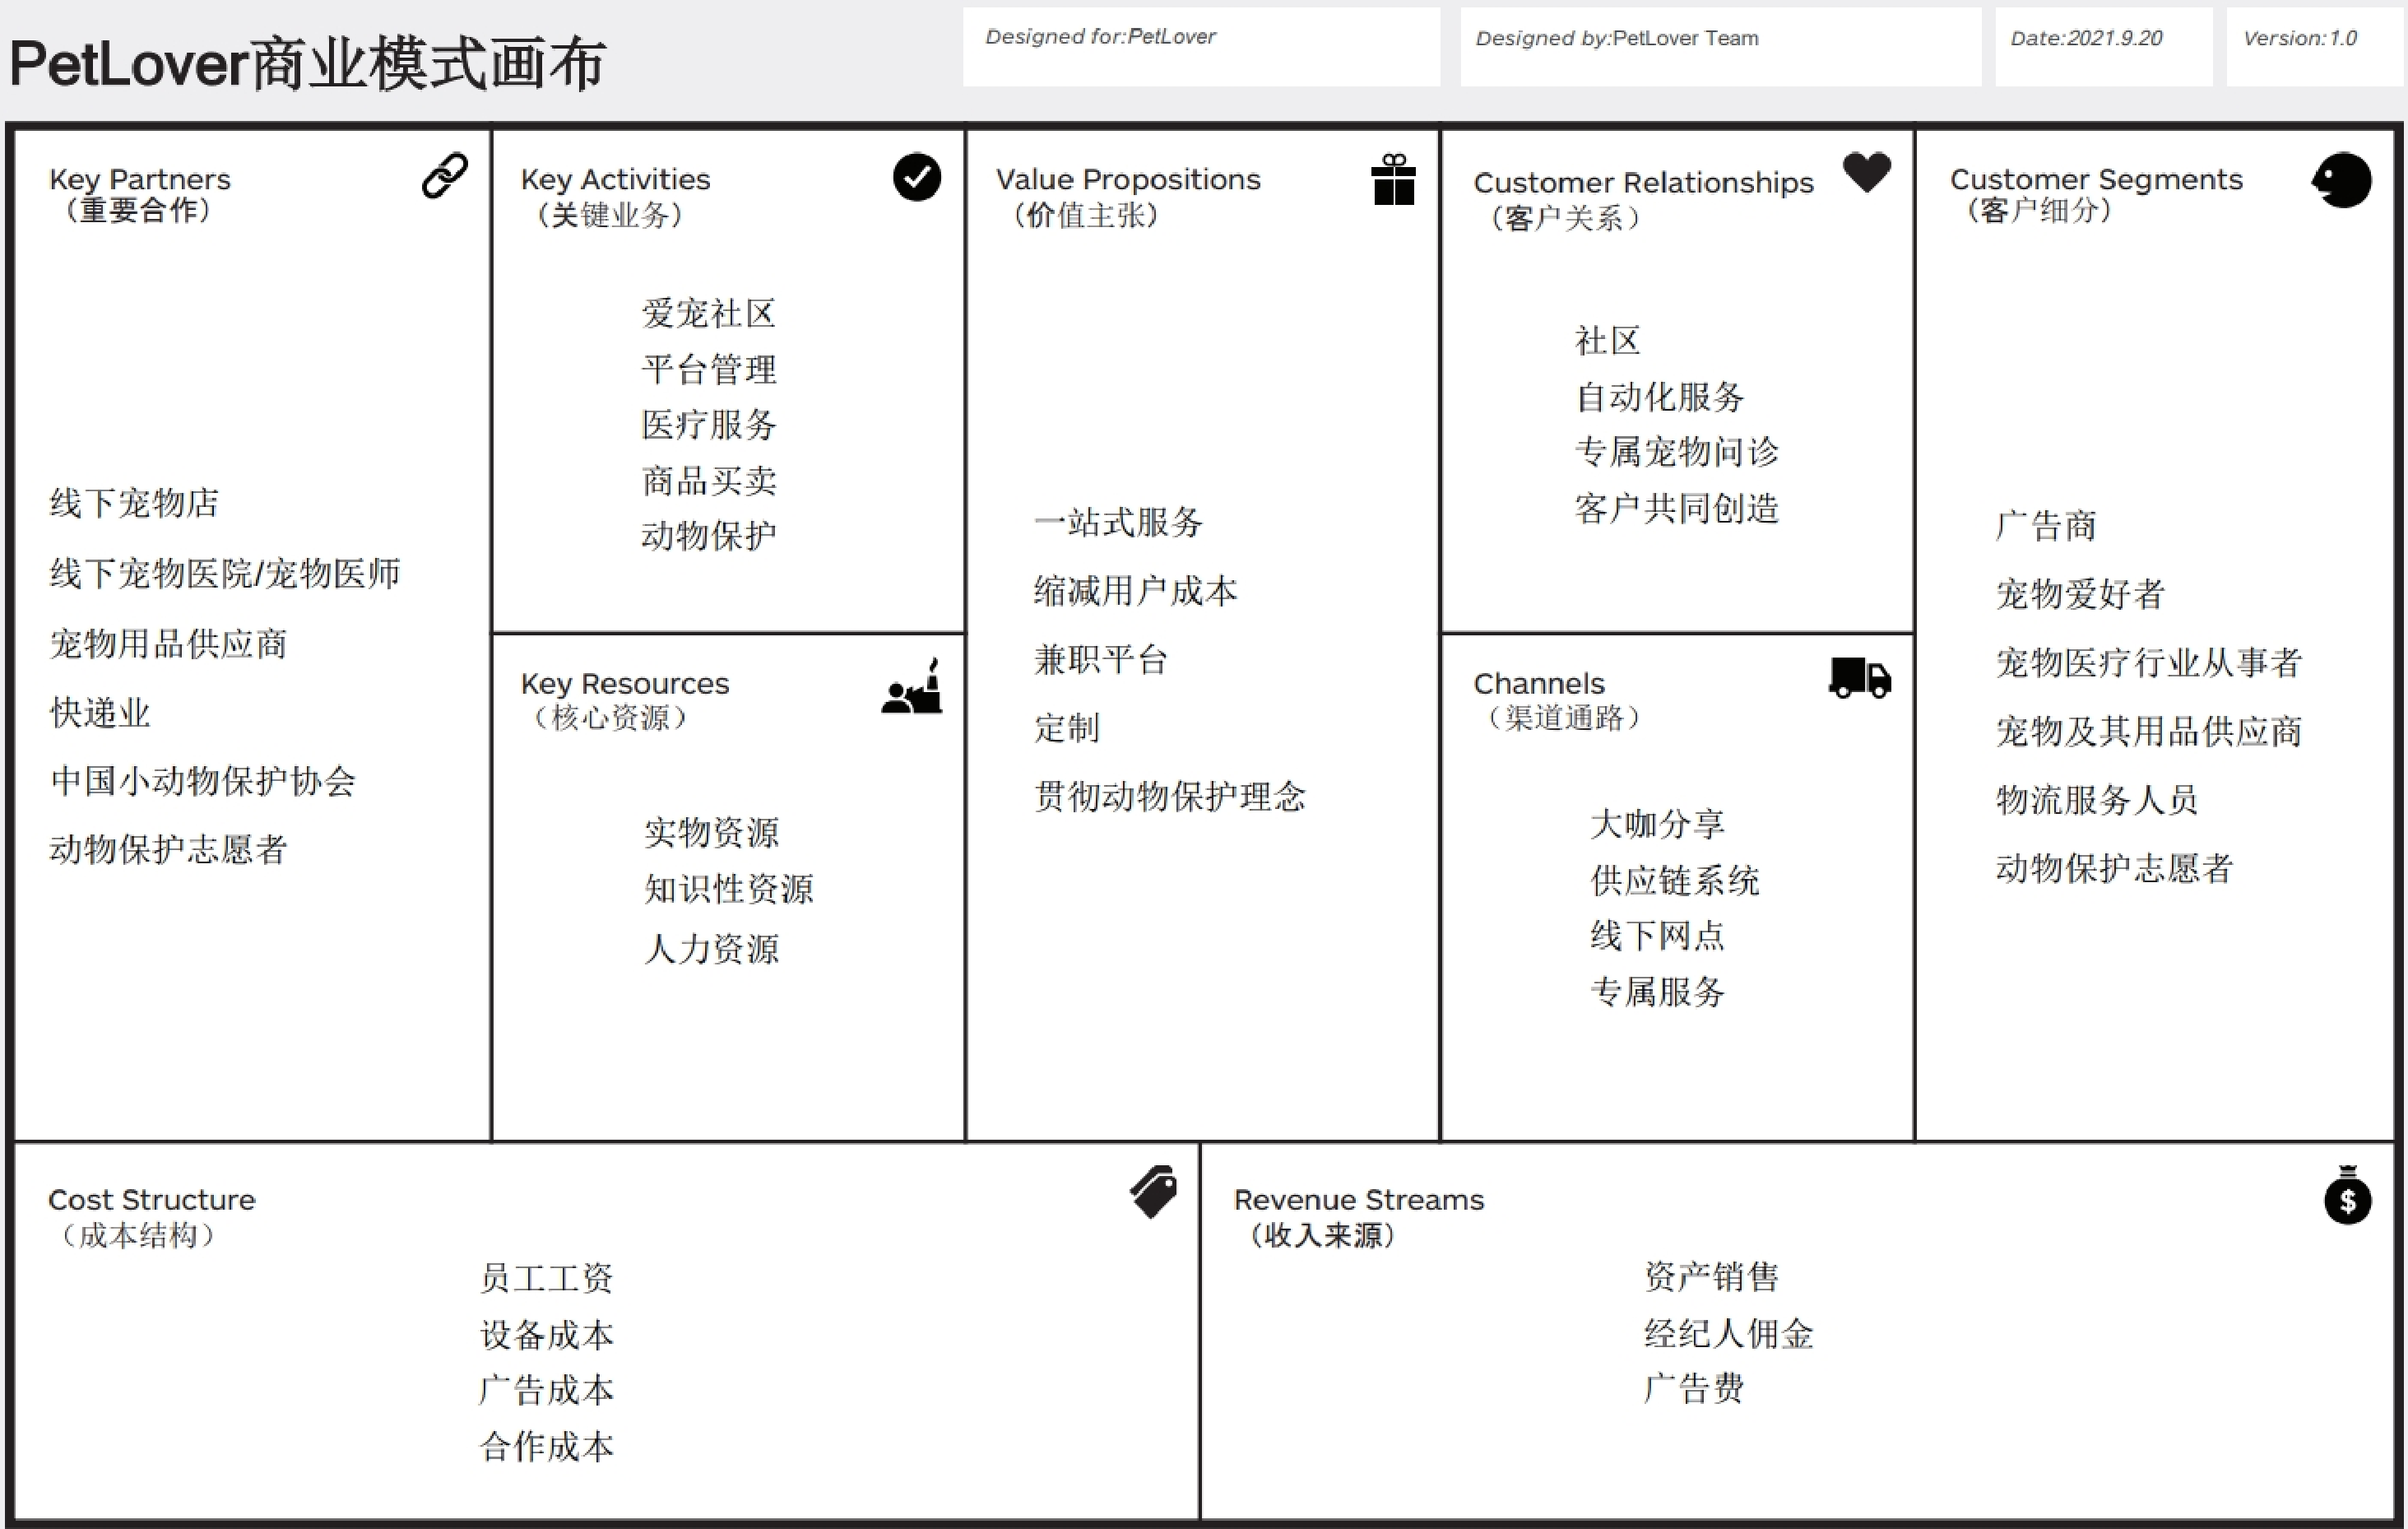
\includegraphics[width=16cm]{the-business-model-canvas}
\end{center}

\subsection{要点介绍}

\subsubsection{关键业务}

\begin{enumerate}[label=\alph*.]
  \item 爱宠社区:为宠物爱好者搭建一个可以交流宠物日常、养宠经验的社区论坛,用户可以通过文字、图片、短视频等媒介在社区中进行日常分享。
  \item 平台管理:PetLover的用户、内容、商品管理都要进行严格把关,保证用户使用体验的良好,保证为用户推荐的内容无不良信息,保证用户本身的纯洁性,清理长期有着不良行为的用户,保证广告商和宠物及供应商的合法性,严格审核加入平台的商家用户。
  \item 医疗服务:提供宠物健康论坛及服务平台,通过宠物健康知识分享、宠物健康咨询、宠物线上问诊、宠物医疗线上预约、宠物药品配送等服务来帮助宠物主人保障爱宠的健康,与各地宠物医院签约并推行该平台作为宠物医院线上问诊的主要平台,为宠物健康撑起一个强有力的保护伞。
  \item 商品买卖:联系各地区宠物或其用品商城使用该平台作为线上交易平台,宠物商品购物网点在全国形成宠物及用品供应网络,同时加强与物流服务公司的合作,为商品买卖提供强大的物流网络,使得商品快速流通来优化用户体验。
  \item 动物保护:获取中国小动物保护协会的许可与授权,吸引动物保护志愿者和自媒体入驻社区论坛,宣传动物保护思想,对于一些可领养城市流浪动物允许志愿者发布流浪动物领养公告,维护小动物的生存权利和不受虐待的权利,改善和提高小动物的生存条件。
\end{enumerate}

\subsubsection{价值主张}

\begin{enumerate}[label=\alph*.]
  \item 一站式服务:实现用户的轻量化操作,为宠物爱好者提供了宠物日常交流、宠物饲养教程、宠物及其用品购买、宠物健康咨询、宠物医疗服务便利的一站式服务,避免宠物爱好者在其他各个服务平台反复切换。
  \item 缩减用户成本:该系统的电商平台为注册宠物用品商家提供补贴,商家无需实体店面,大大缩减了商家用户的经济成本。同时商品种类专门化,买家用户搜索成本大大降低。
  \item 兼职平台:为拥有宠物饲养知识的用户提供通过知识分享获得报酬的机会,为拥有宠物医疗资质的用户提供宠物健康咨询及医治的兼职工作。
  \item 定制:为不同的用户群体定制不同的社区,用户可以根据需求进入不同的社区,如为没有宠物但爱好宠物的用户定制一个关于萌宠视频图片等分享的社区,为拥有宠物的用户定制一个宠物日常分享、宠物饲养技巧、宠物健康问答的社区,为宠物及用品供应商提供各类商品需求、商家售卖心得分享的社区。
  \item 贯彻动物保护理念:动物保护一直以来都是社会的讨论热题,当今社会不乏有故意虐待动物的行为,PetLover平台获得全国小动物保护协会的授权,欢迎动物保护志愿者及相关自媒体入驻社区,创作贯彻珍爱生命、倡导精神文明和发扬人道主义精神理念的作品,坚决反对任何虐待、残害动物的行为和思想。
\end{enumerate}

\subsubsection{客户细分}

\begin{enumerate}[label=\alph*.]
  \item 广告商:投放广告,增加流量。
  \item 宠物爱好者:平台为宠物爱好者(既包括当前已有宠物的群体,也包括由于自身条件如身体条件、住房条件无法饲养宠物或者未来有计划饲养宠物的群体)提供一个可以交流宠物日常的平台,交流的媒介有文字、图片、短视频,他们的身份可以是分享者、提问者和答疑者,答疑者可以通过答疑赚取费用,也可以无偿分享。
  \item 宠物医疗行业从事者:该群体包含宠物医疗服务个体人员和医疗服务中心,他们提供宠物健康咨询建议,分享宠物健康知识,开设宠物饲养教学课程,赚取课程费用;在平台接单来提供线下宠物医疗服务,如上门急救等。
  \item 宠物及其用品供应商:平台保证供应商的出售权利符合相关法律规定,所售商品在法定可售范围内,供应商可以通过交易平台投放自己的商品(如宠物),供其他用户购买,提供商品退换等一系列售后服务。
  \item 物流服务人员:他们一方面为跨城商品运输提供快递配送服务,另一方面为同城商品提供外卖配送服务,在平台收取服务费用,这里的商品指宠物及其用品。
  \item 动物保护志愿者:志愿者可以通过平台宣传动物保护思想,在论坛社区发布城市流浪动物的动态,对于一些可领养城市流浪动物发布流浪动物领养公告。
\end{enumerate}

\subsubsection{客户关系}

\begin{enumerate}[label=\alph*.]
  \item 社区:平台所服务的人群就是宠物相关从业者/爱好者,这些用户群体可以就宠物品种、宠物饲养、宠物诊疗等话题进行讨论,每位用户在相应的讨论中都可以发表自己的见解,共同建立氛围友善的宠物交流社区。
  \item 自动化服务:平台可以根据用户在社区中的相关发言、关注的模块以及已在平台上购买的宠物品种进行宠物(用品)推荐,准时跟进用户需求,并自动推荐相关宠物资源/饲养建议等;或是在购买宠物后,自动推荐该宠物相关的用具/食物购买链接、饲养注意事项等。
  \item 专属宠物问诊:用户可以通过平台的宠物问诊功能获得专属私人服务,咨询宠物医院专业医师获取专业宠物疾病治疗建议。后续治疗过程中,医师也将持续跟进,用户可以在问诊有效期内多次向医师进行咨询。
  \item 客户共同创造:任何用户都可以在平台社区中进行宠物好物分享、产品安利、饲养建议分享等,这些信息对于其他用户的影响,让每位用户都可以在平台上创造资源和使用资源,可以持续推进建设逐渐完善的宠物社区。此外,宠物(及宠物用品)购买者和卖家在交易的过程中,也共同为平台创造了价值。
\end{enumerate}

\subsubsection{核心资源}

\begin{enumerate}[label=\alph*.]
  \item 实物资源:由于平台需要与线下宠物店及宠物医院进行合作,因此需要实体宠物店、宠物医院作实物资源;同时平台支持宠物交易,因此需要销售点管理系统、宠物(及宠物用品)运输系统。
  \item 知识性资源:主要由用户生产的资料组成。包括宠物饲养心得分享、提出的问题及其回答、宠物医师的科普文章等,这些共同组成了平台的知识性资源。
  \item 人力资源:包括软件开发人员和核心用户。平台的开发团队/营销团队、招募的宠物店老板/宠物医师、进行经验分享的知识官等都是平台不可或缺的人力资源。
\end{enumerate}

\subsubsection{重要合作}

\begin{enumerate}[label=\alph*.]
  \item 与线下宠物店的合作:线下宠物店也是平台重要的实物资源,是宠物(及宠物用品)交易的供给侧,也是推进平台持续稳定发展的重要动力。只有与线下宠物店做好合作,才能稳扎稳打推进线上线下并行的交易模式。
  \item 与线下宠物医院/宠物医师的合作:线下宠物医院也是平台重要的实物资源,专业的宠物医师是平台重要的人力资源,也是推进平台持续稳定发展的重要动力,与线下宠物医院/宠物医师积极合作,可以让平台提供宠物疾病针对性的诊疗建议和线下宠物疾病治疗场所。
  \item 与快递业的合作:除线上通过平台预定后进行线下宠物交易外,有些无法前往网点的买家需要选择接收快递的方式,因此,应积极地与快递公司进行合作,并充分考虑宠物运输过程中的安全性、宠物的舒适度、运输速度等因素。对于选择快递收取宠物的买家也要做到充分的保障。
  \item 与宠物用品供应商/采购商的合作:为了保证稳定供应关系,除了与线下宠物店进行合作外,还应与宠物用品供应商/采购商开展合作,保证商品供应链完整、可靠、高效。
  \item 与中国小动物保护协会和动物保护志愿者的合作:为了秉持我们保护动物的价值主张,我们将在社区设立动物保护宣传模块,本平台将获得中国小动物协会的许可和授权,吸引动物保护志愿者和自媒体入驻社区论坛,宣传动物保护思想,贯彻珍爱生命、倡导精神文明和发扬人道主义精神的理念。
\end{enumerate}

\subsubsection{成本结构}

\begin{enumerate}[label=\alph*.]
  \item 员工工资:软件在开发阶段需要有开发人员持续进行开发,软件发布之后需要有客服人员以及维护人员持续提供服务,这些开发与维护人员的薪资均属于不可变的固定成本。
  \item 设备成本:在软件开发初期,一般使用成型的云服务平台,需要支付云服务器的费用。在办公室中还需要支付一定的费用对职员的办公设备进行购买与维护。
  \item 广告成本:在软件宣传的过程中,需要大量的广告宣传来提高知名度,扩充基础个人用户量,维持日活跃用户流量,因此需要提供适当的广告营销成本进行推广。 
  \item 合作成本:为了让平台拥有初始的精品笔记分享、常驻的宠物医师以及宠物店,来打造平台的原生社区环境,还需要支付聘请宠物博主、宠物医师以及加盟宠物店的合作费。
\end{enumerate}

\subsubsection{收入来源}

\begin{enumerate}[label=\alph*.]
  \item 资产销售:平台支持宠物以及宠物用品交易,提供自营店与专卖店,掌握供应链,完善售后客服,提供一系列完整的消费服务,从中收取资产销售费用。
  \item 经纪人佣金:为了方便用户接受线下品牌实体店的服务,平台支持第三方宠物店交易以及宠物医院问诊,在服务过程中提供支付平台,从中收取交易手续费。
  \item 广告费:平台提供一些区域作为发布广告的场所,从广告厂商处收取费用。
\end{enumerate}

\subsubsection{渠道通路}

\begin{enumerate}[label=\alph*.]
  \item 大咖分享:平台通过邀请养宠物的明星、网红等大咖入驻,将宠物的饲养心得、好玩的宠物日常等高质量的原创“安利”内容以笔记的形式在社区发布,使得用户产生信任感与权威感,以达到吸引用户提高知名度的目的。用大咖去吸引用户、链接社群,再用社群绑定用户,做到产品运营、品牌营销、吸粉增粉三者合一。
  \item 供应链系统:平台通过自营旗舰店、国内仓库和线下实体店形成供应链系统。平台的笔记分享能有效帮助用户解决“买什么”“值不值得买”的问题。再结合平台提供的电商系统与供应链系统,使用户能够精确购买,实现评价-购买-传递-售后的一条龙增长,形成社群+电商的商业模式。
  \item 线下网点:平台与线下的宠物店、宠物用品店、宠物医院等达成合作,形成遍布各地的线下网点。在线下网点中,每一个消费者都可以成为品牌和口碑的传播者,最终转变为用户和忠实粉丝。通过线上线下交易一体化的模式,让用户从最初的围观者变为关注者,再从关注者升级为参与者,最后从参与者升级为消费者,形成联动营销模式,实现全渠道的跨界整合。
  \item 专属服务:平台聘请专业宠物医师入驻,对用户提供宠物问诊的专属私人服务,提供专业宠物疾病治疗建议,持续跟进后续治疗,使用户得到满意的服务体验。同时,让用户看着自己的宠物恢复活泼可爱的一面,也将产生强烈的满足感。平台通过专属服务,精准满足用户需求,使用户对平台产生认同感。
\end{enumerate}


\subsection{要点联系}
\subsubsection{2.c(兼职平台)、3.c(宠物医疗行业从事者)、4.c(专属宠物问诊)、9.d(专属服务)}
\paragraph{联系}平台通过认证有从业资格的宠物医疗行业从事者进入平台,提供宠物健康在线咨询服务,收取咨询费用;作为兼职平台令宠物医疗行业从事者利用互联网互联互通优势,持续创造价值。
\subsubsection{2.d(定制)、3.b(宠物爱好者)、4.a(社区)、4.d(客户共同创造)、9.a(大咖分享)}
\paragraph{联系}平台创造定制化社区,邀请养宠物的明星、网红等大咖入驻,提供高质量的社区内容,吸引更多的宠物爱好者反哺社区创造精品内容,不断吸引新的宠物爱好者进入,循换迭代扩大社区体量与质量。
\subsubsection{2.a(缩减用户成本)、9.b(供应链系统)、9.c(线下网点)、3.d(宠物及其用品供应商)、3.d(宠物爱好者)}
\paragraph{联系}在线下网点与各个宠物及其用品供应商建立合作关系,对接平台物流,形成专属稳定的供应链系统。供应商进驻平台可获得优惠补贴,减少商家用户的经济成本。通过平台商品专门化集中化,通过平台自有供应链系统,减少宠物爱好者购买宠物商品的成本。
\subsubsection{2.e(贯彻动物保护理念)、4.a(社区)、3.f(动物保护志愿者)}
\paragraph{联系}平台通过构建公益化的动物保护社区,吸引动物保护志愿者进入,让平台服务中心向外延伸拓展到动物。动物保护志愿者宣传动物保护,得到更多宠物爱好者支持,将理念传播到各个客户细分中。
\subsubsection{2.a(一站式服务)、4.b(自动化服务)、4.c(专属宠物问诊)、9.b(供应链系统)、9.c(线下网点)、9.d(专属服务)3.d(宠物爱好者)}
\paragraph{联系}平台构建与宠物爱好者以自动化服务为代表的成本导向关系以及以专属宠物问诊为代表的价值导向关系,为宠物爱好者提供价格与价值优势。利用供应链系统、线下网点、专属服务渠道落实用户关系,实现一站式服务的价值主张。
\subsubsection{6.b(线下宠物医院/宠物医师)、1.c(医疗服务)}
\paragraph{联系}通过与线下宠物医院/宠物医师合作,支撑起平台关键的宠物医疗服务,让宠物获得线上线下一体的医疗保障。
\subsubsection{6.a(线下宠物店)、6.c(宠物用品供应商)、6.d(快递业)、1.d(商品买卖)}
\paragraph{联系}与各地区线下宠物店与其用品供应商建立合作关系,使用该平台作为线上宠物商品交易平台。同时加强与快递业合作,形成高效快速安全的物流网络,使得商品快速抵达提高用户使用体验。
\subsubsection{6.e(中国小动物保护协会)、6.f(动物保护志愿者)、1.e(动物保护)}
\paragraph{联系}获取中国小动物保护协会的合作认证,吸引动物保护志愿者和自媒体入驻社区论坛。社区动物保护分区宣传动物保护思想,在法律允许的条件下可流浪动物领养公告,改善以宠物为主体的小动物生存条件,扩大动物保护公益事业。
\subsubsection{5.b(知识性资源)、1.a(爱宠社区)、7.c(广告成本)}
\paragraph{联系}用户在社区中发表的精品内容是平台重要的知识性资源。在知识性资源的保障下,爱宠社区形成自己的专业知识壁垒,扩大爱宠社区影响力与知名度,形成社区资源的闭环扩张。为了打造资源富集的社区,需要投放广告来提升社区知名度,吸引优质知识性资源进驻平台。
\subsubsection{4.c(专属宠物问诊)、9.d(专属服务)、8.b(经纪人佣金)}
\paragraph{联系}平台维系专属宠物问诊服务的价值导向关系,提供宠物医生专属服务渠道,从中收取经纪人佣金,使平台获得服务的高价值收入。
\subsubsection{4.b(自动化服务)、9.b(供应链系统)、8.a(资产销售)}
\paragraph{联系}平台获取用户在社区浏览内容、饲养宠物类型、购买过宠物用品等信息,自动推荐用户潜在需要的宠物用品,以强大的自营或第三方知名宠物供应商的供应链系统作为渠道保证,获取资产销售收益,包括平台自营以及第三方平台中介费用。
\subsubsection{4.a(社区)、3.a(广告商)、8.c(广告费)}
\paragraph{联系}平台通过用户体量庞大的社区,为广告商提供用户流量。平台允许优质的广告商以软广告推荐的方式进入社区,平台从中获取广告费用。
\subsubsection{1.b(平台管理)、5.c(人力资源)、7.a(员工工资)}
\paragraph{联系}平台需要软件运维人员和平台与社区管理人员等人力资源,做到平台功能稳定、社区内容健康积极高质量、平台推荐商品质量有保障等平台管理关键业务。这样的人员工资开销构成了平台主要的成本开销。
\subsubsection{1.c(医疗服务)、4.d(商品买卖)、5.a(实物资源)、7.d(合作成本)}
\paragraph{联系}为了维持平台的宠物医疗服务和宠物商品销售业务,平台需要宠物医院、宠物店、宠物用品供应商等线下实物资源来维护平台的资源壁垒和不可替代性。因此平台需要支付合作的线下实体资源优惠等合作成本来维护平台的不可替代性。
\subsubsection{6.a(线下宠物店)、6.b(线下宠物医院/宠物医师)、9.c(线下网点)}
\paragraph{联系}平台需要加强和线下宠物店以及线下宠物医院/宠物医师的合作,才能通过实体设施维护和客户的线下网点的渠道通路良好运转。
\subsubsection{6.c(宠物用品供应商)、6.d(快递业)、9.b(供应链系统)}
\paragraph{联系}平台把线下宠物用品实体店作为商品供应节点,与稳定的快递业合作形成商品快速流通网络,作为供应链系统的重要环节。
\subsubsection{6.a(线下宠物店)、6.b(线下宠物医院/宠物医师)、6.c(宠物用品供应商)、6.d(快递业)、5.a(实物资源)}
\paragraph{联系}平台需要维持与宠物店、宠物医院/宠物医师、宠物用品供应商、快递业等重要合作,构建平台的实物资源,支持平台服务的稳定可靠运营。
\subsubsection{2.a(一站式服务)、3.b(宠物爱好者)、2.c(兼职平台)、3.c(宠物医疗从业者)、8.b(经纪人佣金)}
\paragraph{联系}包含宠物健康咨询的一站式服务为宠物爱好者提供高价值私人服务;宠物医疗从业者进驻作为兼职平台利用零碎时间额外产生价值。平台通过这两个主张和客户细分从中获取经纪人佣金。
\end{document}